\chapter{Oracle Aplication Express}

\section{Tahapan Pembuatan Aplikasi Oracle Apex}
Langkah pertama yang harus dilakukan untuk bisa masuk ke dalam oracle apex online adalah membuat akun terlebih dahulu kemudia login pada website https://apex.oracle.com, disini  akan mendapatkan akses untuk memasuki Oracle Apllication Express, pastikan email yang dimasukkan valid untuk membuat Workspace, berikut adalah langkah langkah pembuatan Aplikasi pada Oracle APEX :

\begin{enumerate}
\item[1]Pergi ke Website Oracle APEX, https://apex.oracle.com, lalu klik Sign In.

\begin{figure}[!htbp]
    \begin{center}
    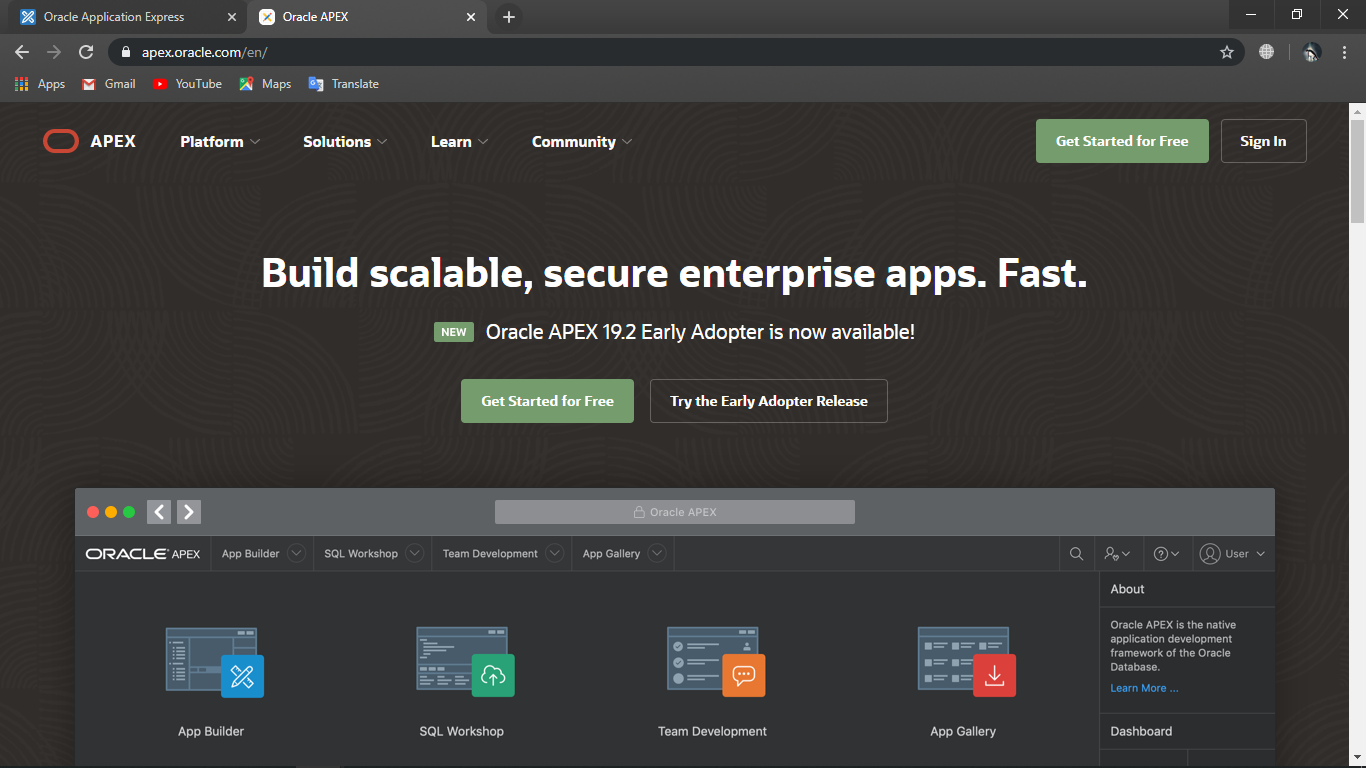
\includegraphics[scale=0.4]{figures/14.png}
    \caption{\textit{Sign In.}}
    \end{center}   
    \end{figure}
    
\begin{figure}[!htbp]
\item[2]Lalu Masukan Workspace yang telah dibuat sebelumnya.

    \begin{center}
    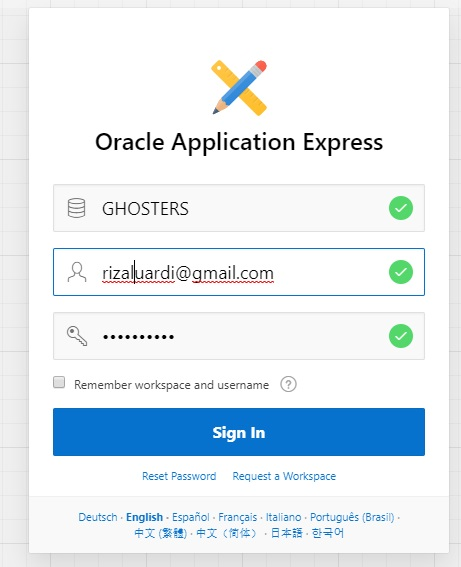
\includegraphics[scale=0.5]{figures/2.jpg}
    \caption{\textit{Sign In Workspace.}}
    \end{center}


\item[3] Lalu setelah Sign In, Klik App Builder .

    \begin{center}
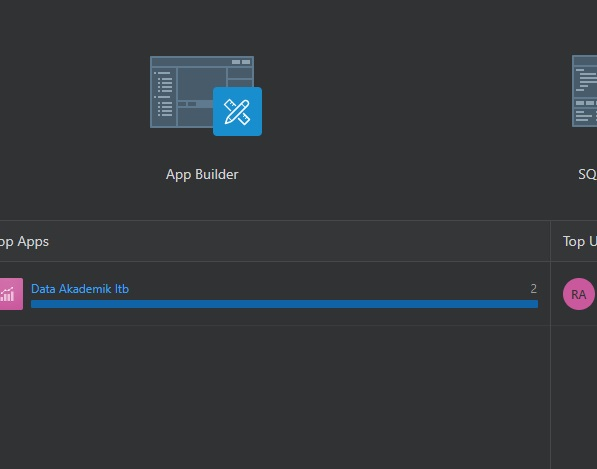
\includegraphics[scale=0.5]{figures/3.jpg}
    \caption{\textit{App Builder}}
        \end{center}
\label{gambar}
\end{figure}

\begin{figure}
\item[4] Setelah di klik App Builder, lalu Akan muncul Create, Klik Create.

    \begin{center}
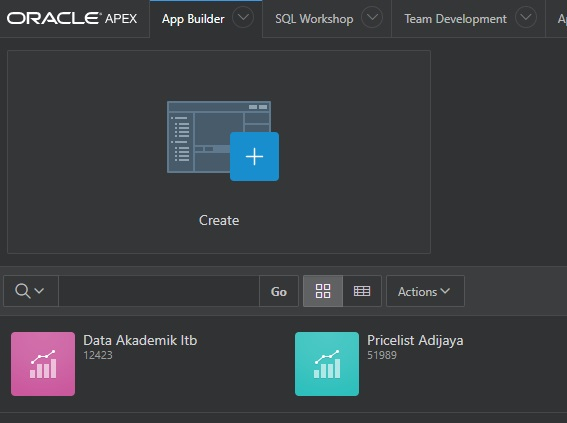
\includegraphics[scale=0.4]{figures/4.jpg}
    \caption{\textit{Create .}}
        \end{center}
\label{gambar}
\end{figure}

\begin{figure}
\item[5] Setelah di klik Create,Lalu Klik From a File .

    \begin{center}
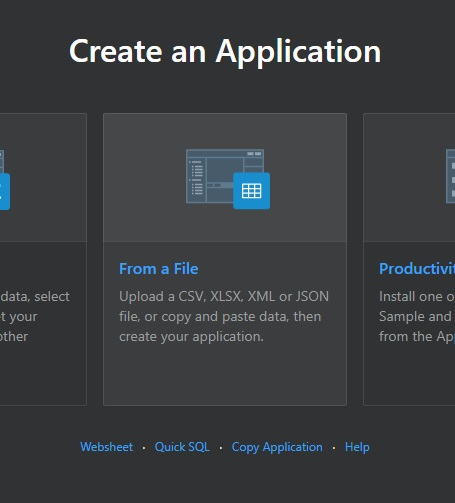
\includegraphics[scale=0.4]{figures/5.jpg}
    \caption{\textit{{Proses Input Data Excel}l}}
        \end{center}
\label{gambar}
\end{figure}

\begin{figure}
\item[6] Masukan data excel yang akan digunakan untuk membuat aplikasi.

    \begin{center}
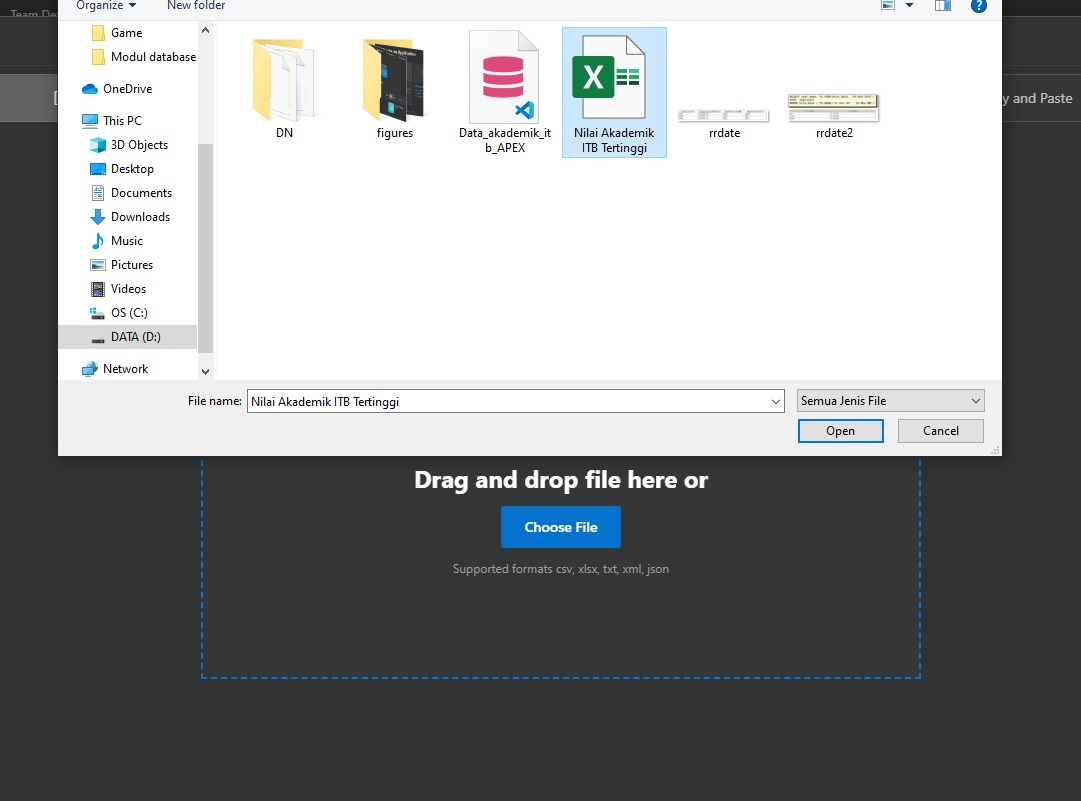
\includegraphics[scale=0.4]{figures/6.jpg}
    \caption{\textit{Input Data Excel.}}
        \end{center}
\label{gambar}
\end{figure}

\begin{figure}
\item[7] Lalu Muncul Tampilan seperti ini. Di Table Nama saya beri PENDAFTARAN MAHASISWA.

    \begin{center}
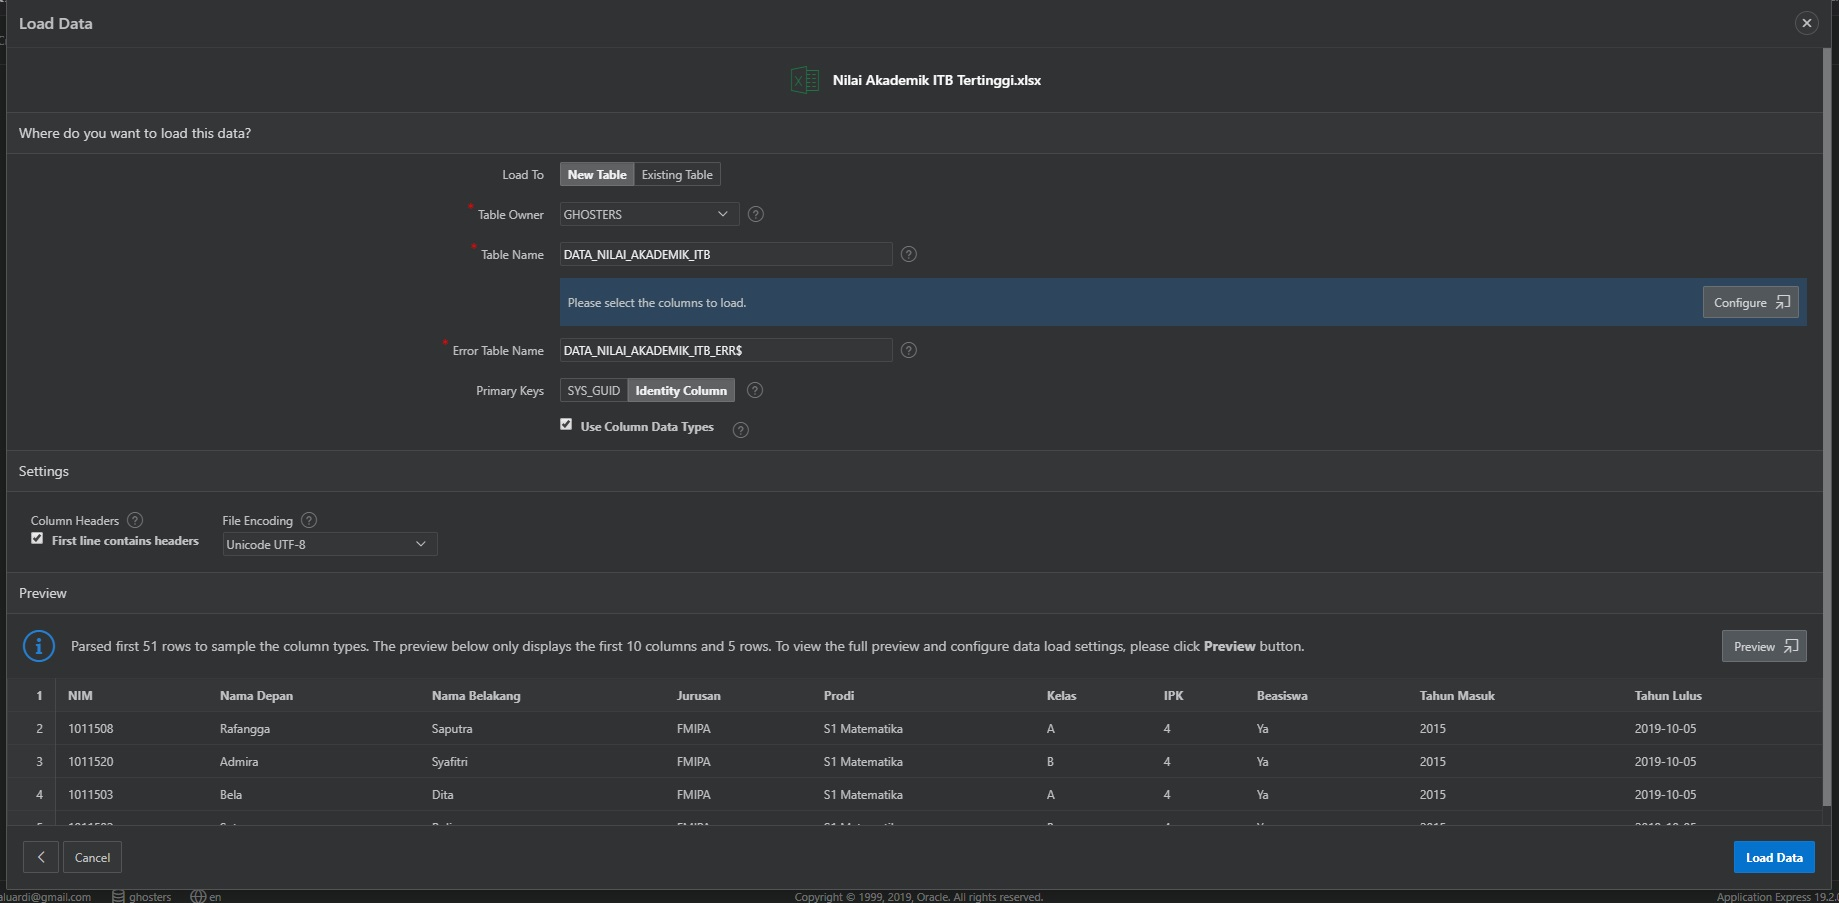
\includegraphics[scale=0.2]{figures/7.jpg}
    \caption{\textit{Pengisian Nama Table}}
        \end{center}
\label{gambar}
\end{figure}

\begin{figure}
\item[8] Proses Pembuatan Aplikasi Berhasil.

    \begin{center}
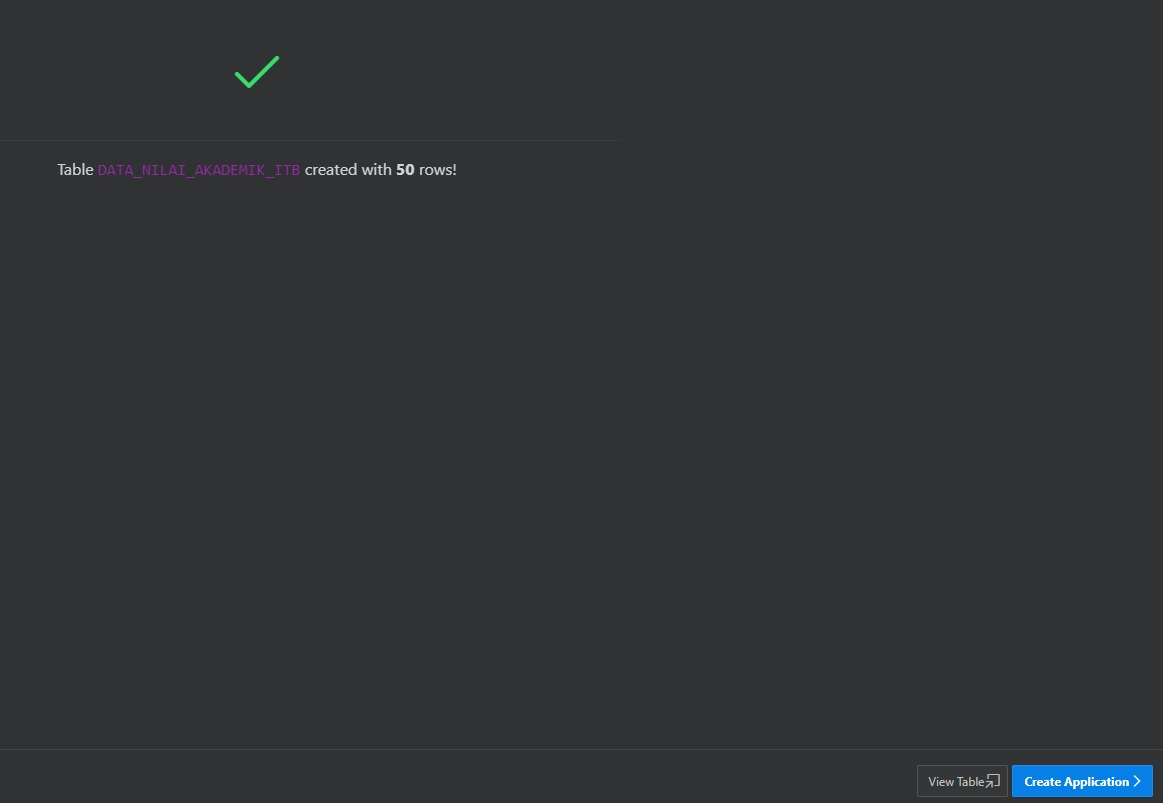
\includegraphics[scale=0.2]{figures/8.jpg}
    \caption{\textit{Aplikasi Berhasil}}
        \end{center}
\label{gambar}
\end{figure}

\begin{figure}
\item[9] Klik Create Application .

    \begin{center}
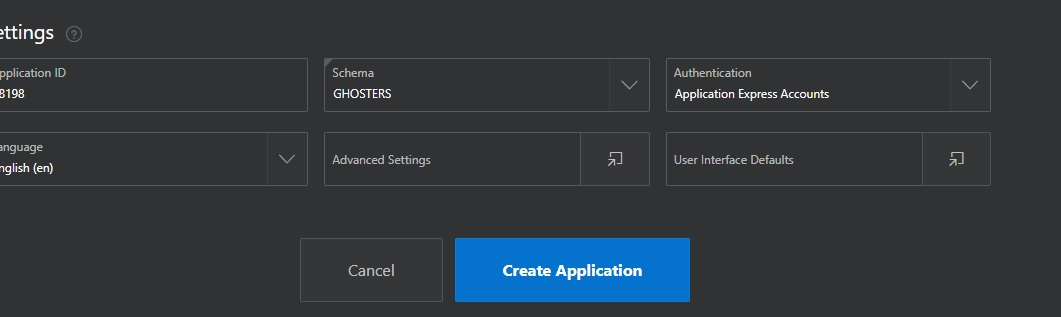
\includegraphics[scale=0.2]{figures/9.jpg}
    \caption{\textit{Create Application}}
        \end{center}
\label{gambar}
\end{figure}

\begin{figure}
\item[10] Lalu Klik Run.
    \begin{center}
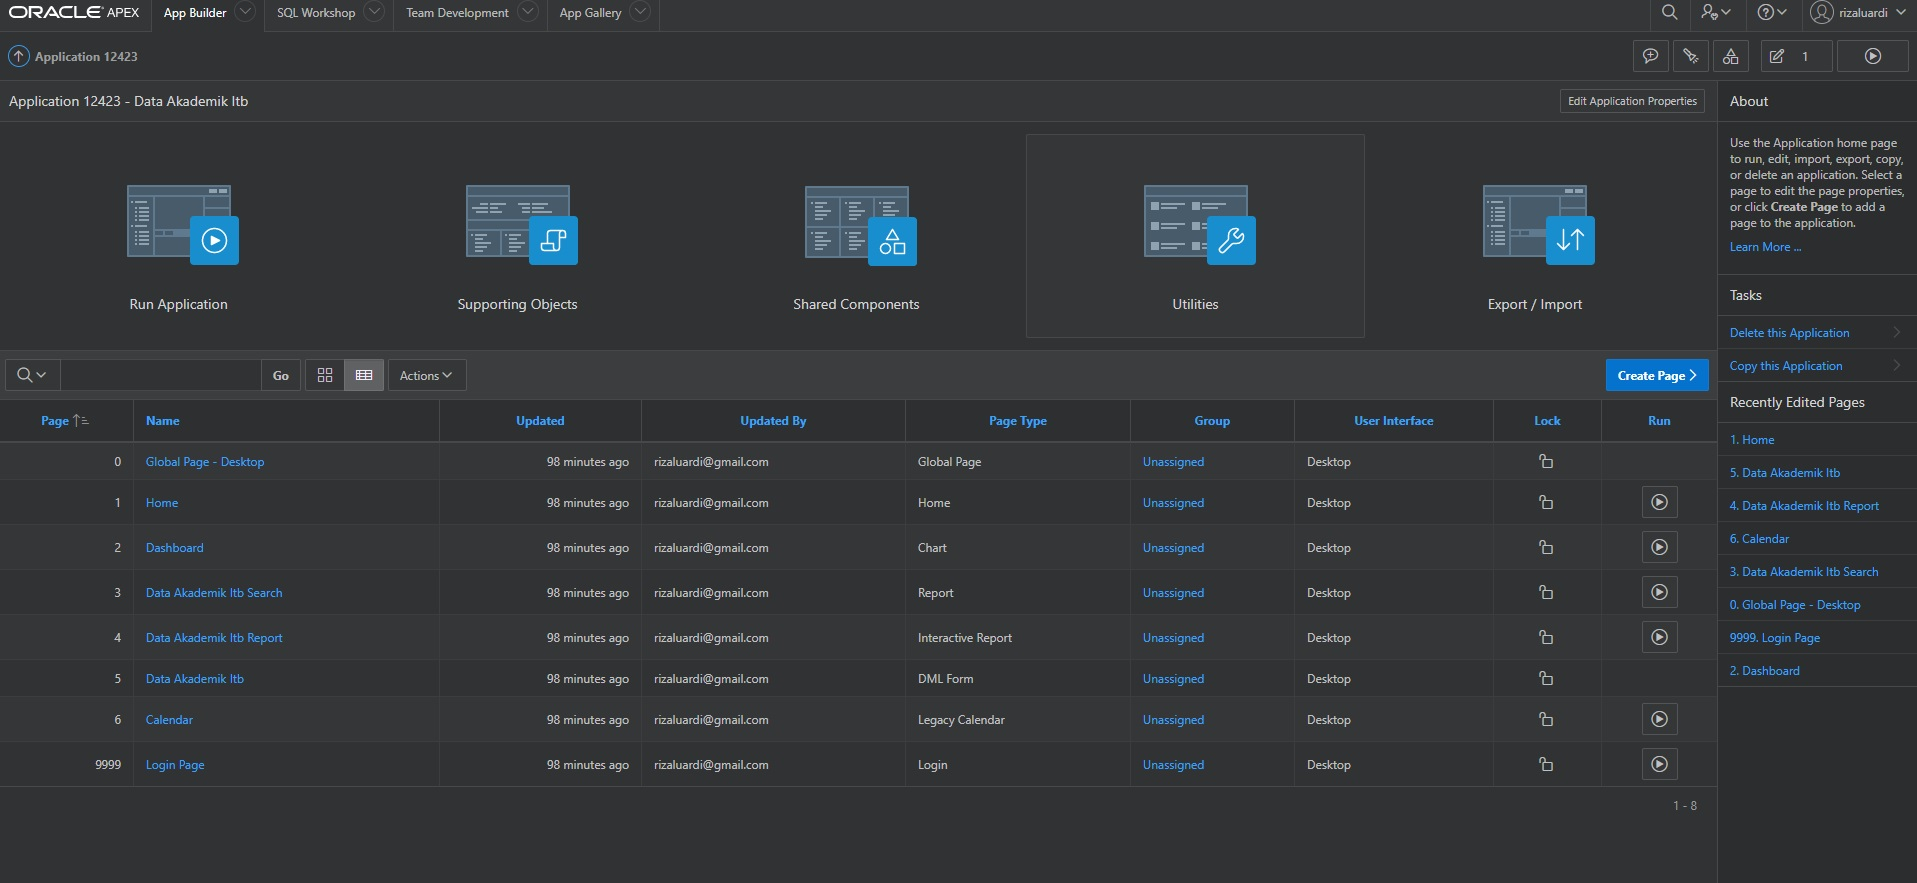
\includegraphics[scale=0.2]{figures/10.jpg}
    \caption{\textit{Run}}
        \end{center}
\label{gambar}
\end{figure}

\begin{figure}
\item[11] Lalu Masukan email sama password yang telah dibuat.

    \begin{center}
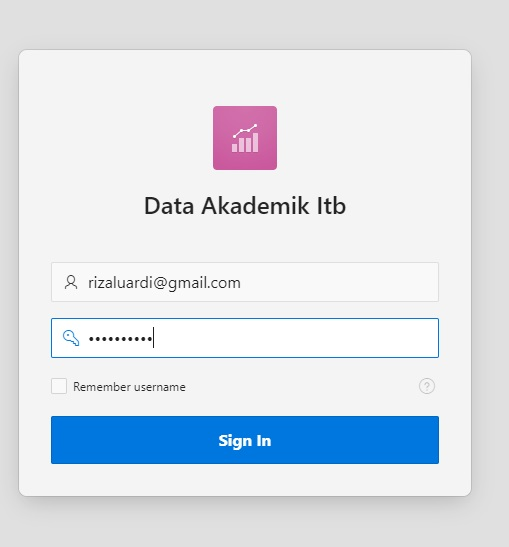
\includegraphics[scale=0.4]{figures/11.jpg}
    \caption{\textit{Masukan Email}}
        \end{center}
\label{gambar}
\end{figure}

\begin{figure}
\item[12] Lalu akanmuncul tampilan seperti ini.

    \begin{center}
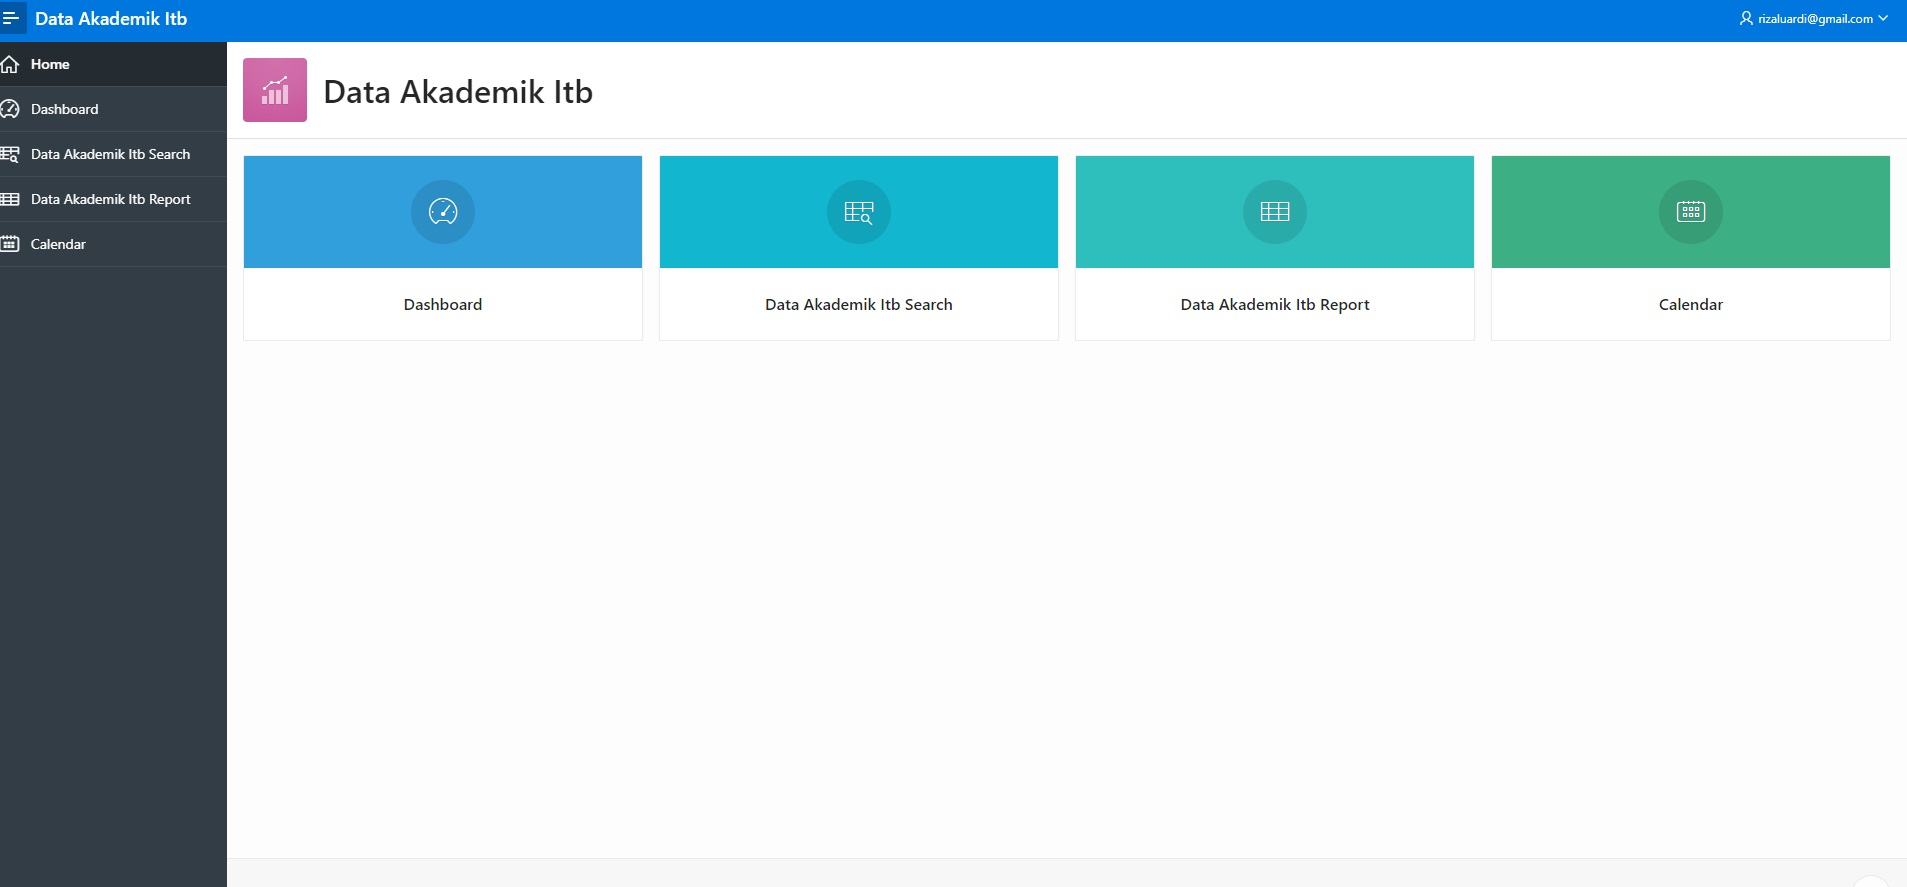
\includegraphics[scale=0.2]{figures/12.jpg}
    \caption{\textit{Tampilan Berhasil.}}
        \end{center}
\label{gambar}
\end{figure}

\begin{figure}
\item[13] Link,user,dan kata sandi ada di gambar berikut
    \begin{center}
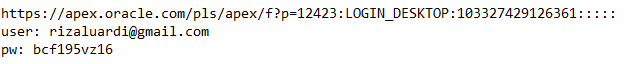
\includegraphics[scale=0.2]{figures/13.png}
    \caption{\textit{Tampilan LINK dan user.}}
        \end{center}
\label{gambar}
\end{figure}

    

\end{enumerate}
